% *********************************************************************
% © 2010–2022 Jeremy Sylvestre
%
% Permission is granted to copy, distribute and/or modify this document
% under the terms of the GNU Free Documentation License, Version 1.3 or
% any later version published by the Free Software Foundation; with no
% Invariant Sections, no Front-Cover Texts, and no Back-Cover Texts. A
% copy of the license is included in the appendix entitled “GNU Free
% Documentation License” that appears in the output document of this
% PreTeXt source code. All trademarks™ are the registered® marks of
% their respective owners.
%
% *********************************************************************

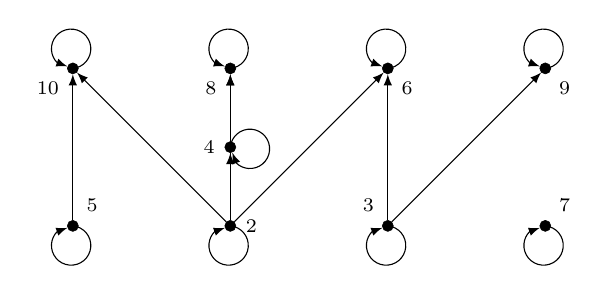
\begin{tikzpicture}[
	vertex/.style={ circle, draw, very thin, fill, inner sep=0pt, minimum size=4pt },
	vertexg/.style={ black!40!white, circle, draw, very thin, fill, inner sep=0pt, minimum size=4pt },
	vertexo/.style={ circle, draw, very thin, inner sep=0pt, minimum size=4pt }
]

\node at (2,2) (six) [vertex,label=below right:$\scriptstyle 6$] {};
\draw[-latex] (six) arc (-85:225:0.25cm) to (six);
\node at (4,2) (nine) [vertex,label=below right:$\scriptstyle 9$] {};
\draw[-latex] (nine) arc (-85:225:0.25cm) to (nine);
\node at (0,1) (four) [vertex,label=left:$\scriptstyle 4$] {};
\draw[-latex] (four) arc (175:-135:0.25cm) to (four);
% \draw[-latex] (four) arc (-85:225:0.25cm) to (four);
\node at (-2,2) (ten) [vertex,label=below left:$\scriptstyle 10$] {};
\draw[-latex] (ten) arc (-85:225:0.25cm) to (ten);
\node at (0,2) (eight) [vertex,label=below left:$\scriptstyle 8$] {};
\draw[-latex] (four) to (eight);
\draw[-latex] (eight) arc (-85:225:0.25cm) to (eight);
\node at (0,0) (two) [vertex,label=right:$\scriptstyle 2$] {};
\foreach \p in {six,four,eight,ten} \draw[-latex] (two) to (\p);
\draw[-latex] (two) arc (85:-225:0.25cm) to (two);
\node at (2,0) (three) [vertex,label=above left:$\scriptstyle 3$] {};
\foreach \p in {six,nine} \draw[-latex] (three) to (\p);
\draw[-latex] (three) arc (85:-225:0.25cm) to (three);
\node at (4,0) (seven) [vertex,label=above right:$\scriptstyle 7$] {};
\draw[-latex] (seven) arc (85:-225:0.25cm) to (seven);
\node at (-2,0) (five) [vertex,label=above right:$\scriptstyle 5$] {};
\draw[-latex] (five) to (ten);
\draw[-latex] (five) arc (85:-225:0.25cm) to (five);

\end{tikzpicture}
